\subsubsection{UCA 5 - Monitoraggio dello storico degli accessi dell'utente}

\begin{figure}[h]
	\centering	
	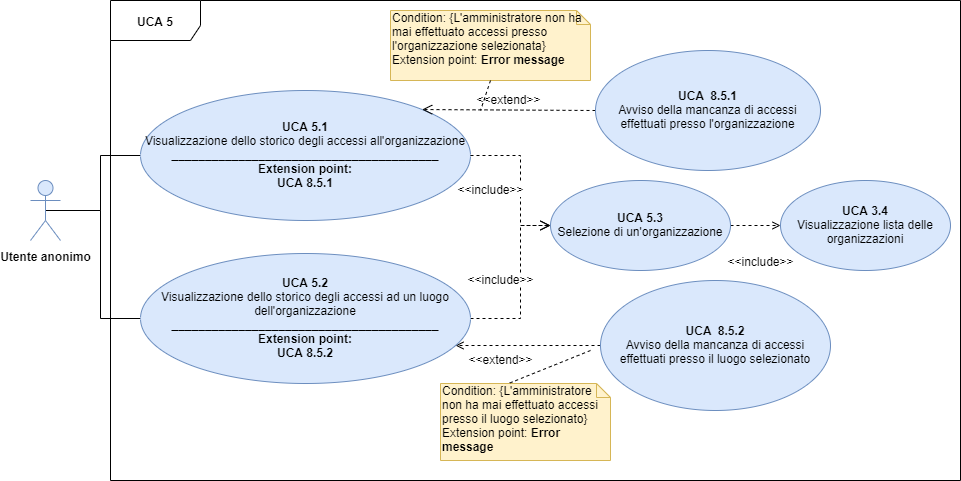
\includegraphics[scale=0.4, center]{Sezioni/UseCase/Immagini/UCA5.png}
	\caption{UCA 5 - Monitoraggio dello \glo{storico degli accessi} dell'utente}
\end{figure}

\begin{itemize}
    \item \textbf{Attori primari:} Utente anonimo
    \item \textbf{Precondizione:} L'utente ha precedentemente scaricato la lista delle \glo{organizzazioni}.
    \item \textbf{Postcondizione:} L'utente ha visualizzato lo \glo{storico degli accessi} relativo all'\glo{organizzazione} desiderata oppure al \glo{luogo} desiderato dell'\glo{organizzazione} scelta.
    \item \textbf{Scenario principale:} L'utente selezionerà l'\glo{organizzazione} desiderata dalla lista delle \glo{organizzazioni} e quindi la funzionalità per mostrare lo \glo{storico degli accessi} oppure un \glo{luogo} specifico per analizzarne il relativo \glo{storico degli accessi}.
\end{itemize}

\subsubsection{UCA 5.1 - Visualizzazione dello storico degli accessi all'organizzazione}
\begin{itemize}
    \item \textbf{Attori primari:} Utente anonimo
    \item \textbf{Precondizione:} L'utente ha precedentemente scaricato la lista delle \glo{organizzazioni}.
    \item \textbf{Postcondizione:} L'utente ha visualizzato lo \glo{storico degli accessi} (con nome dell'\glo{organizzazione}, \glo{timestamp} di ingresso, di uscita, e tempo di permanenza) presso l'\glo{organizzazione} scelta. Se si trova all'interno dell'\glo{organizzazione} stessa, viene visualizzato il tempo passato al suo interno dall'ultimo ingresso effettuato.
    \item \textbf{Scenario principale:} L'utente esegue la procedura per visualizzare lo \glo{storico degli accessi} effettuati presso l'\glo{organizzazione} desiderata.
    \item \textbf{Scenario alternativo:} L'utente non è mai entrato nell'\glo{organizzazione} selezionata, pertanto verrà visualizzato un avviso informativo [UCA 8.5.1].
    \item \textbf{Flusso di eventi:}
    \begin{enumerate}
        \item L'utente seleziona l'\glo{organizzazione} interessata [UCA 5];
        \item L'utente seleziona la funzionalità per mostrare gli accessi effettuati presso l'\glo{organizzazione} selezionata;
        \item L'utente ha la possibilità di ordinare gli accessi all'\glo{organizzazione} [UCA 5.1.1] [UCA 5.1.2] oppure di effettuare una ricerca tra di essi per gli accessi di uno specifico giorno [UCA 5.1.3].
    \end{enumerate}
    \item \textbf{Inclusioni:}
    \begin{itemize}
        \item UCA 5.3 - Selezione di un'\glo{organizzazione}.
    \end{itemize}
    \item \textbf{Estensioni:}
    \begin{itemize}
        \item UCA 8.5.1 - Avviso della mancanza di accessi effettuati presso l'organizzazione selezionata.
    \end{itemize}
\end{itemize}

\subsubsection{UCA 5.1.1 - Ordinamento per data decrescente della lista degli accessi presso un'organizzazione}
\begin{itemize}
	\item \textbf{Attori primari:} Utente anonimo
	\item \textbf{Precondizione:} L'utente sta visualizzando lo storico accessi di un'\glo{organizzazione} [UCA 5].
	\item \textbf{Postcondizione:} L'utente ottiene la \glo{lista degli accessi} riordinata \glo{per data in ordine decrescente}.
	\item \textbf{Scenario principale:} Ordinamento per data decrescente della lista degli accessi presso un'organizzazione.
	\item \textbf{Flusso di eventi:}
	\begin{enumerate}
		\item L'utente seleziona la funzionalità per riordinare lo \glo{storico degli accessi} dell'\glo{organizzazione}\glo{per data in ordine decrescente}.
	\end{enumerate}   
\end{itemize}

\subsubsection{UCA 5.1.2 - Ordinamento per data crescente della \glo{lista degli accessi} presso un'organizzazione}
\begin{itemize}
	\item \textbf{Attori primari:} Utente anonimo
	\item \textbf{Precondizione:} L'utente sta visualizzando lo \glo{storico degli accessi} di un'\glo{organizzazione} [UCA 5].
	\item \textbf{Postcondizione:} L'utente ottiene la \glo{lista degli accessi} riordinata \glo{per data in ordine crescente}.
	\item \textbf{Scenario principale:} Ordinamento per data crescente della \glo{lista degli accessi} presso un'organizzazione.
	\item \textbf{Flusso di eventi:}
	\begin{enumerate}
		\item L'utente seleziona la funzionalità per riordinare lo \glo{storico degli accessi} dell'\glo{organizzazione} \glo{per data in ordine crescente}.
	\end{enumerate}
\end{itemize}

\subsubsection{UCA 5.1.3 - Ricerca degli accessi presso un'organizzazione in un giorno specifico}
\begin{itemize}
	\item \textbf{Attori primari:} Utente anonimo
	\item \textbf{Precondizione:} L'utente sta visualizzando lo storico accessi di un'\glo{organizzazione} [UCA 5].
	\item \textbf{Postcondizione:} L'utente ottiene la \glo{lista degli accessi} effettuati nel giorno selezionato.
	\item \textbf{Scenario principale:} Ricerca degli accessi presso un'organizzazione in un giorno specifico.
	\item \textbf{Flusso di eventi:}
	\begin{enumerate}
		\item L'utente seleziona la funzionalità per visualizzare solo gli accessi avvenuti in un giorno specifico presso l'\glo{organizzazione};
		\item L'utente seleziona il giorno desiderato.
	\end{enumerate}  
\end{itemize}

\subsubsection{UCA 5.2 - Visualizzazione dello storico degli accessi ad un luogo dell'organizzazione}
\begin{itemize}
    \item \textbf{Attori primari:} Utente anonimo
    \item \textbf{Precondizione:} L'utente sta visualizzando lo storico accessi di un'\glo{organizzazione} [UCA 5] e l'\glo{organizzazione} in questione deve avere almeno un \glo{luogo} registrato.
    \item \textbf{Postcondizione:} L'utente visualizza lo \glo{storico degli accessi} (con nome del \glo{luogo}, \glo{timestamp} di ingresso, di uscita, e tempo di permanenza) al \glo{luogo} desiderato. Se l'utente dovesse trovarsi all'interno del \glo{luogo} stesso, viene visualizzato il tempo passato al suo interno dall'ultimo ingresso effettuato.
    \item \textbf{Scenario principale:} L'utente esegue la procedura per visualizzare lo \glo{storico degli accessi} effettuati presso il \glo{luogo} desiderato.
    \item \textbf{Scenario alternativo:} L'utente non è mai entrato nel \glo{luogo} selezionato, pertanto verrà mostrato un avviso informativo [UCA 8.5.2].
    \item \textbf{Flusso di eventi:}
    \begin{enumerate}
        \item L'utente seleziona l'\glo{organizzazione} interessata [UCA 5.3];
        \item L'utente seleziona un \glo{luogo} tra quelli offerti dall'\glo{organizzazione} selezionata;
        \item L'utente seleziona la funzionalità per mostrare gli accessi effettuati presso il \glo{luogo} selezionato;
        \item L'utente ha la possibilità di ordinare gli accessi al \glo{luogo} [UCA 5.2.1] [UCA 5.2.2] oppure di effettuare una ricerca tra di essi per gli accessi di uno specifico giorno [UCA 5.2.3].
    \end{enumerate}
    \item \textbf{Inclusioni:}
    \begin{itemize}
        \item UCA 5.3 - Selezione di un'organizzazione.
    \end{itemize}
    \item \textbf{Estensioni:}
    \begin{itemize}
        \item UCA 8.5.2 - Avviso della mancanza di accessi effettuati presso il luogo selezionato.
    \end{itemize}
\end{itemize}

\subsubsection{UCA 5.2.1 - Ordinamento per data decrescente della lista degli accessi presso un luogo di un'organizzazione}
\begin{itemize}
    \item \textbf{Attori primari:} Utente anonimo
    \item \textbf{Precondizione:} L'utente sta visualizzando lo storico accessi di un \glo{luogo} [UCA 5.1].
    \item \textbf{Postcondizione:} L'utente ottiene la \glo{lista degli accessi} riordinata \glo{per data in ordine decrescente}.
    \item \textbf{Scenario principale:} Ordinamento per data decrescente della lista degli accessi presso un luogo di un'organizzazione.
    \item \textbf{Flusso di eventi:}
    \begin{enumerate}
        \item L'utente seleziona la funzionalità per riordinare lo \glo{storico degli accessi} del \glo{luogo} \glo{per data in ordine decrescente}.
    \end{enumerate}
\end{itemize}

\subsubsection{UCA 5.2.2 - Ordinamento per data crescente della lista degli accessi presso un luogo di un'organizzazione}
\begin{itemize}
    \item \textbf{Attori primari:} Utente anonimo
    \item \textbf{Precondizione:} L'utente sta visualizzando lo storico accessi di un \glo{luogo} [UCA 5.1].
    \item \textbf{Postcondizione:} L'utente ottiene la lista degli iniziale riordinata \glo{per data in ordine crescente}.
    \item \textbf{Scenario principale:} Ordinamento per data crescente della lista degli accessi presso un luogo di un'organizzazione.
    \item \textbf{Flusso di eventi:}
    \begin{enumerate}
        \item L'utente seleziona la funzionalità per riordinare lo \glo{storico degli accessi} del \glo{luogo} \glo{per data in ordine crescente}.
    \end{enumerate}
\end{itemize}

\subsubsection{UCA 5.2.3 - Ricerca degli accessi presso un luogo di un'organizzazione in un giorno specifico}
\begin{itemize}
    \item \textbf{Attori primari:} Utente anonimo
    \item \textbf{Precondizione:} L'utente sta visualizzando lo storico accessi di un \glo{luogo} [UCA 5.1].
    \item \textbf{Postcondizione:} L'utente ottiene la \glo{lista degli accessi} effettuati presso il \glo{luogo} in questione nel giorno selezionato.
    \item \textbf{Scenario principale:} Ricerca degli accessi presso un luogo di un'organizzazione in un giorno specifico.
    \item \textbf{Flusso di eventi:}
    \begin{enumerate}
        \item L'utente seleziona la funzionalità per visualizzare solo gli accessi avvenuti in un giorno specifico presso il \glo{luogo} in questione dell'\glo{organizzazione};
        \item L'utente seleziona il giorno desiderato.
    \end{enumerate}
\end{itemize}

\subsubsection{UCA 5.3 - Selezione di un'organizzazione}
\begin{itemize}
    \item \textbf{Attori primari:} Utente anonimo
    \item \textbf{Precondizione:} L'utente ha precedentemente scaricato la lista delle \glo{organizzazioni}.
    \item \textbf{Postcondizione:} L'utente ha selezionato un'\glo{organizzazione} dalla lista.
    \item \textbf{Scenario principale:} L'utente selezionerà l'\glo{organizzazione} desiderata dalla lista delle \glo{organizzazioni}.
    \item \textbf{Flusso di eventi:}
    \begin{enumerate}
        \item L'utente visualizza la lista delle \glo{organizzazioni} [UCA 3.4];
        \item L'utente seleziona dalla lista l'\glo{organizzazione} interessata.
    \end{enumerate}
    \item \textbf{Inclusioni:}
    \begin{itemize}
        \item UCA 3.4 - Visualizzazione lista delle organizzazioni.
    \end{itemize}
\end{itemize}